\documentclass[conference]{IEEEtran}
\IEEEoverridecommandlockouts
% The preceding line is only needed to identify funding in the first footnote. If that is unneeded, please comment it out.
\usepackage{cite}
\usepackage{amsmath,amssymb,amsfonts}
\usepackage{algorithmic}
\usepackage{graphicx}
\usepackage{textcomp}
\usepackage{xcolor}
\def\BibTeX{{\rm B\kern-.05em{\sc i\kern-.025em b}\kern-.08em
    T\kern-.1667em\lower.7ex\hbox{E}\kern-.125emX}}
    
% Code formatting
\usepackage{listings}
\usepackage{xcolor}

\definecolor{codegreen}{rgb}{0,0.6,0}
\definecolor{codegray}{rgb}{0.5,0.5,0.5}
\definecolor{codepurple}{rgb}{0.58,0,0.82}
\definecolor{backcolour}{rgb}{0.95,0.95,0.92}

\lstdefinestyle{cpp}{
    backgroundcolor=\color{backcolour},
    commentstyle=\color{codegreen},
    keywordstyle=\color{magenta},
    numberstyle=\tiny\color{codegray},
    stringstyle=\color{codepurple},
    basicstyle=\ttfamily\footnotesize,
    breakatwhitespace=false,
    breaklines=true,
    captionpos=b,
    keepspaces=true,
    numbers=left,
    numbersep=5pt,
    showspaces=false,
    showstringspaces=false,
    showtabs=false,
    tabsize=2
}

\lstset{style=cpp}
    

\begin{document}

\title{Concurrent Graph Algorithms}

\author{\IEEEauthorblockN{Jacob Steinebronn}
\and
\IEEEauthorblockN{Daniel West}
\and
\IEEEauthorblockN{William Quiroga}
\and
\IEEEauthorblockN{Alex Rutledge}}

\maketitle

\begin{abstract}
This project does a shallow dive into concurrent implementation in c++ for 4 graph topics: All-Pairs-Shortest-Path, the Disjoint Set Union data structure, Minimum-Spanning-Tree, and Single-Source-Shortest-Path. Implementations take both correctness and running-time into account, and are benchmarked on a 12-core, 24-thread machine. 
\end{abstract}

\begin{IEEEkeywords}
graph, algorithm, dijkstra, floyd-warshall, shortest-path
\end{IEEEkeywords}

\section{Introduction}
In this paper, we will perform a wide analysis on several high-level graph topics: the All-Pairs-Shortest-Path problem, the Minimum Spanning Tree problem, the Shortest-Distance problem with negative edges, and the Disjoint Set Union data structure (which is often used in graph algorithms such as connectivity or Kruskal's MST algorithm). In particular, the implementations of these algorithms in parallel will be analyzed in detail regarding the best practices for different use-cases or input regimes. 
\section{All-Pairs Shortest-Path}

\subsection{Problem Definition}

Given a weighted, undirected graph G, $\forall u, v \in G$, find $DIST_{u,v}$ equal to the shortest path in G from $u$ to $v$. In general, the edge weights can be any real number, but for our purposes it will be convenient to restrict edge weights to non-negative integers which do not exceed $10^9$. This will be done for two main reasons:
\begin{itemize}
    \item To restrict the maximum possible answer into an integer which can be stored conveniently in most modern operating systems (a 64-bit signed integer will suffice)
    \item To restrict the graph such that path lengths are defined. With negative edge weights, a path could simply traverse this negative edge back and forth infinitely many times, so any fully relaxed path in a graph with at least one negative edge weight will have all paths of length $-\infty$
\end{itemize}
These two items let us prove a convenient upper-bound on the length of any one shortest path as follows: Let $w_{max}$ be the largest possible edge weight. Any shortest path from $u$ to $v$, $P = p_0,p_1,...p_{n-1},p_k \,\,|\,\, p_0 = u, p_k = v$ will be simple; that is, there will not exist any node $p_i$ which appears in $P$ twice. We can show this by contradiction: If there were some node that appeared twice in $P$, let the first and last occurrence of this duplicate node be $p_i$ and $p_j$, then $P' = p_0, p_1...p_i,p_{j+1},p_{j+2}...p_k$ would be shorter. That is, we could "cut out" the cycle between $p_i$ and $p_j$. Thus, we know that for any shortest path, every node in G will appear at most once, so the maximum value for any shortest path in a graph of $n$ nodes is $n * w_{max}$.

\subsection{Sequential Implementations}
We will examine two implementations for the All-Pairs-Shortest-Path problem: the Floyd-Warshall algorithm, and All-Sources Dijkstra's algorithm. While these algorithms are well-known, we will enumerate the specific implementations in c++ we'll be building off in the future. 

\lstinputlisting[
    language=C++,
    caption=Sequential Dijkstra's on Adjacency Matrix,
    label=lst:seqdijkstra
]{./src/APSP/dijkstra.cpp}

\lstinputlisting[
    language=C++,
    caption=Sequential Floyd-Warshall's on Adjacency Matrix,
    label=lst:seqfloyds
]{./src/APSP/floyds.cpp}

These are the most basic implementations of both Dijkstra's and Floyd-Warshall's. Note that the Dijkstra's implementation has been adapted to write its output into the pre-defined matrix *res* and called on every start point (Since Dijkstra's algorithm calculates Single-source Shortest-Path to all nodes). As a sanity-check, we run these implementations on the CSES (Code Submission Evaluation System) set "Shortest Routes II", and they of course pass. The Dijkstra's implementation is $\mathcal{O}(n^3\log{}n)$, and the Floyd's implementation is $\mathcal{O}(n^3)$. Sequentially, Floyd's is faster in every case due to its superior time-complexity and extremely low overhead; however, when both algorithms for APSP are adapted to be run non-sequentially, we'll see that this is no longer *always* true. 

\subsection{Floyd-Warshall's Algorithm in Parallel}
Perhaps the most straightforward attempt at parallelizing the Floyd-Warshall algorithm would be to split up the outermost for loop (the "K loop"), and dividing the execution of this outer loop (and of course, the corresponding execution of the inner loops) evenly among the threads. Such an implementation would look as follows:

\lstinputlisting[
    language=C++,
    caption=Incorrect attempt at parallelizing Floyd's,
    label=lst:badfloyds
]{./src/APSP/floyds_bad.cpp}

It isn't too hard to see why this is wrong: semantically, the "K loop" is iterating over all paths of length 2 that pass through one node called the "pivot", and performing edge relaxations over that pivot. However, when multiple pivots are being simultaneously processed, a situation could arise where a node which is a pivot in one thread has an edge relaxation happen over it, which disturbs the value of any future relaxations with that pivot by introducing a circular dependency in the relaxations. Indeed, it is not hard to generate graphs for which this implementation is correct; suffice it to say, this approach is incorrect.

The initial approach, while it was wrong, did give some hints as to a way to correctly parallelize Floyd-Warshall's algorithm. Instead of splitting up the outermost "K loop", we can split up the middle "I loop" instead for each k. This works correctly, since every relaxation over a single pivot operates independently. In fact, even without a proof of correctness for the Floyd-Warshall algorithm or knowing how it works, this can be observed simply from the code shown in Listing 2. All 5 of the array lookups and the array update are only operating on either row $adj[i]$ or $adj[k]$, so the only issue any thread would have performing an entire pass through the "I loop" would be if an update to $adj[k]$ was an update on $adj[i]$; that is, if for some relaxation inside the "K loop", node k had an edge relaxation. However, since k is the pivot, any relaxation would do nothing, since $adj[k][k] = 0$. Thus, every thread's work is independent of every other thread. So an algorithm to run Floyd's in parallel would be to iterate the outer loop sequentially, and then spawn new threads for every outer iteration to complete every middle and inner loop in parallel:

\break

\begin{figure}[t]
    \lstinputlisting[
        language=C++,
        caption=Correct attempt at parallelizing Floyd's,
        label=lst:spawnfloyds
    ]{./src/APSP/floyds_spawn.cpp}
\end{figure}

Indeed, generating and testing this implementation (Which we'll call "Floyd's Spawn" since it spawns new worker threads for each iteration) against random graphs, and comparing the output to the Dijkstra's and Floyd's implementations shown in Figures 1 and 2 shown to be correct, this works as intended. 

\begin{figure}[t]
    \centering
    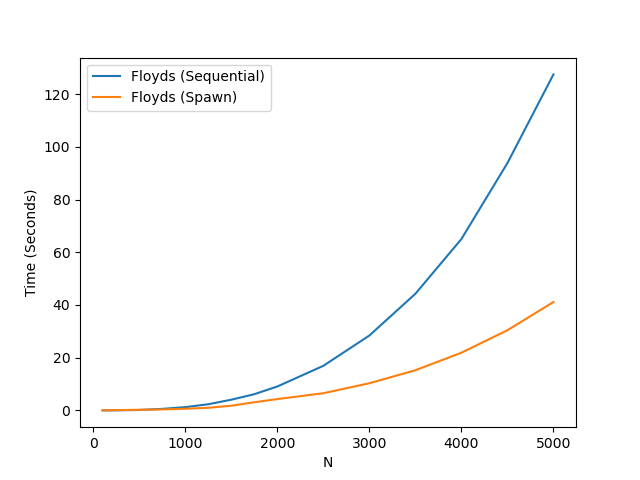
\includegraphics[width=9cm]{images/benchspawn2.png}
    \caption{Parallel Floyd's-Spawn with 20 threads versus sequential Floyd's}
    \label{fig:floyds_spawn}
\end{figure}

We can observe in figure \ref{fig:floyds_spawn} a roughly 3x speedup with 20 threads with this method. We will go in greater detail with the effects of thread count on running time later. 

The main potential problem with this solution is the overhead of repeatedly creating and destroying threads for every iteration of the "K loop". We can fix this problem by creating the worker threads once and re-using them, but we will have to make sure that one worker thread does not move ahead to the next value of k before every other thread has finished with the same thread. We can accomplish this by having each thread increment a counter when it finishes for some k, and then wait (by locking a mutex). Then, when this counter reaches the number of threads, every thread can be unlocked and continue on to the next value of k. This process will repeat for $n$ iterations. We will call this approach "Floyd's-Sync", since all the threads are "syncing" before moving on together to the next value of k (after which they might fall out of sync until finishing). The c++ implementation for this approach is shown in listing \ref{lst:syncfloyds}.

\begin{figure}[t]
    \lstinputlisting[
        language=C++,
        caption=Floyd's-Sync implementation,
        label=lst:syncfloyds
    ]{./src/APSP/floyds_sync.cpp}
\end{figure}

\begin{figure}[t]
    \centering
    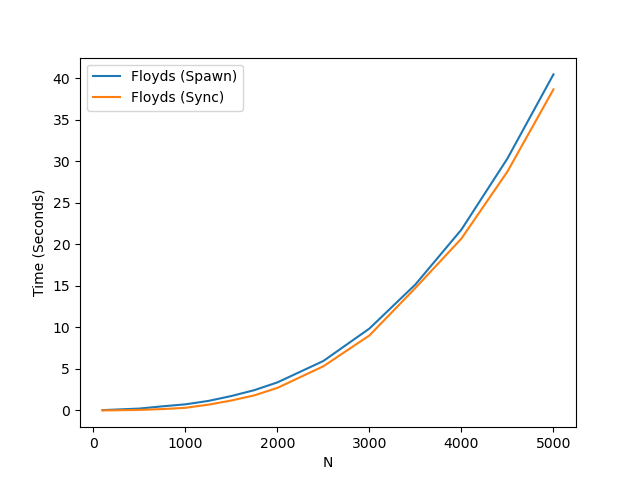
\includegraphics[width=9cm]{images/benchsync.png}
    \caption{Floyd's-Sync versus Floyd's-Spawn, both with 20 threads}
    \label{fig:floyds_both}
\end{figure}


Again, running this implementation against the others which are working as intended, this implementation also produces correct output. Figure \ref{fig:floyds_both} shows Floyd's-Sync and Floyd's-Spawn run on the same inputs, and while the improvement is only marginal, Floyd's-Sync is consistently slightly faster than Floyd's-Spawn.

\subsection{Dijkstra's Algorithm in Parallel}\label{AA}
In the previous section, we analyzed different practices for computing the All-Pairs-Shortest-Path matrix in parallel using Floyd-Warshall's algorithm. The other algorithm we will be considering for computing this matrix will be All-Sources Dijkstra's algorithm; that is, we will run Dijkstra's from every node as a source. If we observe the implementation shown in listing \ref{lst:seqdijkstra}, we will notice that, for any function call of $dijkstra$ on an arbitrary starting point $s$, the only changes that can be seen from outside the method are in the row $res[s]$. This suggests an implementation of All-Sources Dijkstra's in parallel: Call $dijkstra(i)$ on every node. As observed previously, we won't have any issues like we had in the previous section with Floyd's, as any updates are constrained to a single row in the result matrix, and function calls to $dijkstra$ are ambivalent to any changes made in any row except for the row of the starting node. Thus, we do not expect any issues, and can code a relatively straightforward parallelization shown in listing \ref{lst:pqdijkstras}.

\begin{figure}[t]
    \lstinputlisting[
        language=C++,
        caption=Trivial Dijkstra's parallelization,
        label=lst:pqdijkstras
    ]{./src/APSP/dijkstra_pq.cpp}
\end{figure}

\begin{figure}[t]
    \centering
    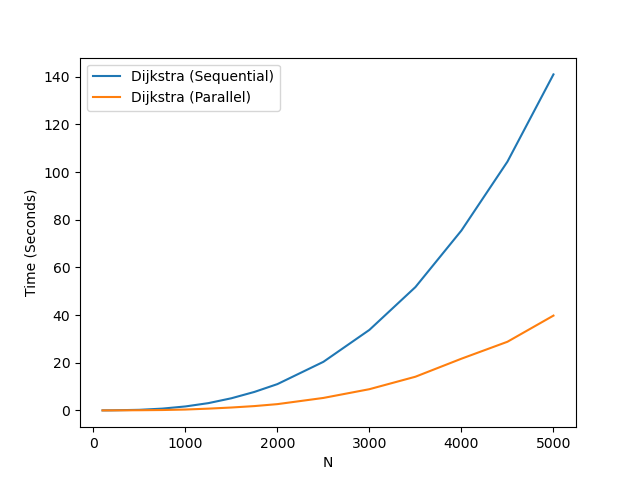
\includegraphics[width=9cm]{images/benchpq.png}
    \caption{Sequential vs Parallel Dijkstra's APSP with 20 threads}
    \label{fig:dijkstra_pq}
\end{figure}

Note, this is on randomly-generated graphs (Still within the restrictions outlined earlier). We will analyze the running time of this implementation against an adversarial graph later. 

\break
\break

\begin{figure}[t]
    \lstinputlisting[
        language=C++,
        caption=Dijkstra's with Linear Search instead of Priority Queue
        label=lst:lineardijkstras
    ]{./src/APSP/dijkstra_linear.cpp}
\end{figure}


% t(top) h(here) b(bottom)
\begin{figure}[h]
    \centering
    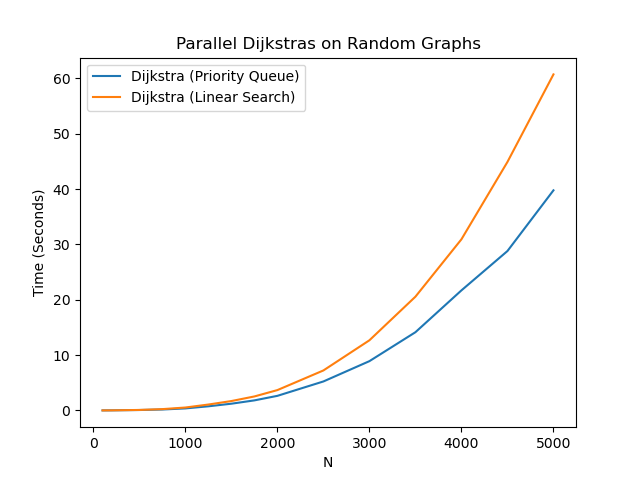
\includegraphics[width=9cm]{images/benchdijkstra.png}
    \caption{Dijkstra's with Priority Queue vs Dijkstra's with Linear Search on randomly-generated graphs, both with 20 threads}
    \label{fig:dijkstra_both}
\end{figure}

\subsection{Parallel Dijkstra's Algorithm Performance in the Worst Case}\label{AA}
The above results, showing that parallel Dijkstra's with a priority queue for selecting states performs better than using a linear search when the input is a randomly-generated graph (Still within the restrictions outlined earlier). On randomly-generated graphs, we can expect the size of the priority queue to be quite small, since a large majority of the graphs would have edges which are far greater in weight than some shortest path which could circumvent that edge; thus, the number of new states which repeat on unexplored nodes would be low. In fact, the size of the priority queue can be observed to be $O(n)$ on random graphs. However, if we have an adversarial-generated graph, one where the particular implementation of priority-queue Dijkstra's is taken into account, we can get this priority queue to grow with the number of edges in the graph, which is $O(n^2)$. 

Performing a rough analysis of the linear-search versus the priority-queue implementations will illuminate the running time in the average (random graph) versus worst(adversarial graph) case. The linear search implementation always takes exactly $2n^2$ per Dijkstra's call: For each of $i$ iterations, do a single loop of size $n$ to find the source, and then another loop of size $n$ to perform relaxations. This is the same regardless of the graph itself because the edge weights do not affect the time it takes to update the $res$ array or perform the first loop to find the source. However, for the priority-queue implementation, the edge weights strongly influence the running-time in that they influence the size of the priority queue used to find the source for each iteration. In a random graph, the size of the priority queue is expected to be roughly linear, since the expected number of edges in a path is very small. We perform n removals from the priority queue, each of which takes $O(log(n))$, and n insertions, each of which also takes $O(log(n))$. Thus, in the average case, the expected number of operations is roughly $n*log(n) + n*log(n) + n^2$ which is strongly dominated by $n^2$. However, in the worst case, the size of the priority queue is $O(n^2)$; thus, the number of insertions is $n^2$, each taking $log(n^2) = 2log(n)$, so the number of operations in the worst case for this implementation is roughly $2n^2*log(n)$ which, compared to the worst-case for linear search Dijkstra's, is worse by an entire log factor, not to mention the overhead of actually maintaining the priority queue rather than the extremely low-overhead for loop. 

We can improve upon this worst-case runtime in Dijkstra's by making an observation about the priority queue iteself: There are many states inside the priority queue which are contributing to the runtime of adding/removing to the queue that aren't even useful. Consider a graph with 3 nodes $u,v,w$ and a BFS-ordering $u,v,w$: node $u$ will place nodes $v$ and $w$ into the priority queue, then node $v$ might put node $w$ into the queue again, so now node $w$ is in the queue twice, even though only one of the states is actually the minimal distance. We can fix this by instead of maintaining a priority queue of states, we can maintain an ordered set of them. Then, when we want to update the distance of a state, we can remove the old entry in the set for that state, having found a better one, before inserting the new one. That way, even if every node in the graph can be found in the "queue" at one time, it will appear only once, so the size of the "queue" is bounded by $n$ instead of $n^2$. We will still have a worst-case number of insertions being $n^2$, but at least we can speed up the insertions/removals by a factor of two. This can be observed in Fig. \ref{fig:dijkstra_all}

\begin{figure}[t]
    \lstinputlisting[
        language=C++,
        caption=Dijkstra's with Ordered Set instead of Priority Queue
        label=lst:setdijkstras
    ]{./src/APSP/dijkstra_set.cpp}
\end{figure}

\begin{figure}[h]
    \centering
    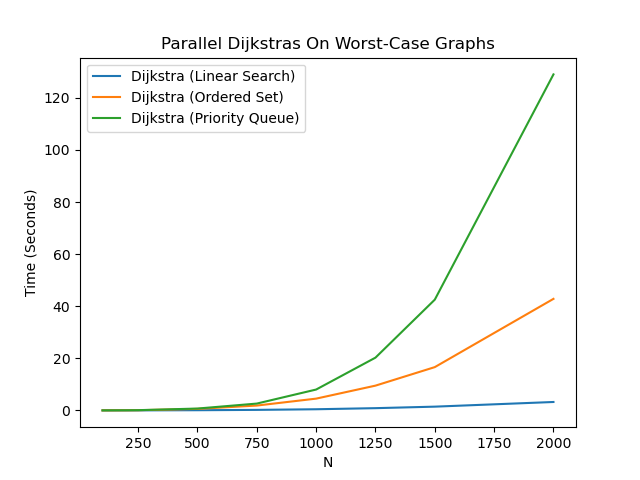
\includegraphics[width=9cm]{images/benchWorstCase2.png}
    \caption{Various Parallel Dijkstra's implementations on worst-case graphs}
    \label{fig:dijkstra_all}
\end{figure}



\section{Minimum Spanning Tree}
The Minimum Spanning Tree (MST) problem is a common architecture building problem that finds the minimum-weighted connected graph of a certain set of connected vertices\cite{b2}. The graph will contain V-1 edges where V is the total number of vertices in the graph. This problem can be found in many real life problems such as road construction, circuit design \& development, and phone line planning. In the realm of computer science research the MST problem can also be used to approximate NP-Hard problems such as the traveling salesperson\cite{b1}. We will be looking at how to properly implement a solution concurrently and compare the runtimes to the sequential implementation.
\par

\subsection{Prim's MST}
Prim's MST is a greedy approach to the MST problem where the concept is to maintain two sets of vertices: the set of vertices included in the tree, and the vertices yet to be added. As the tree is built, each edge between the two sets are considered and the smallest weighted edge is chosen to be a part of the tree. The minKey function takes in the two sets and returns the index of the minimum weighted edge that connects the two. The sequential implementation can be seen below:

\lstinputlisting[
    language=C++,
    caption=,
    label=,
]{./src/MST/prims_seq.cpp}

Since the edges of the spanning tree need to be added sequentially, the algorithm contains only two highly parallelizable sections of code: the minKey function and the comparison of edge weights in the inner loop of the primMST function.
\newpage
\lstinputlisting[
    language=C++,
    caption=,
    label=,
]{./src/MST/prims_minkey.cpp}
\subsection{Parallelization}
The minKey function as shown above can be parallelized by dividing the for loop into subsections and storing the minimum key for a thread locally and comparing these minimums when the threads close.

\lstinputlisting[
    language=C++,
    caption=,
    label=,
]{./src/MST/prims_minkey_par.cpp}

This implementation sustains the correctness of the minKey function in that it will always select the minimum key within the proper set of vertices, but because this is a parallel implementation it is possible that this function will produce a different minKey index than it's sequential counterpart. Therefore, the correctness of the sequential and parallel programs was checked by comparing the total weights of each spanning tree rather than checking which edges were included.
\par
The second point of parallelization comes in the primMST function after the minKey function:

\lstinputlisting[
    language=C++,
    caption=,
    label=,
]{./src/MST/prims_par.cpp}
\subsection{Test Data}

Run-time testing was done on a 12-core CPU, and each test iteration was done with 10 total tests with incremental input sizes.

\begin{figure}[h]
    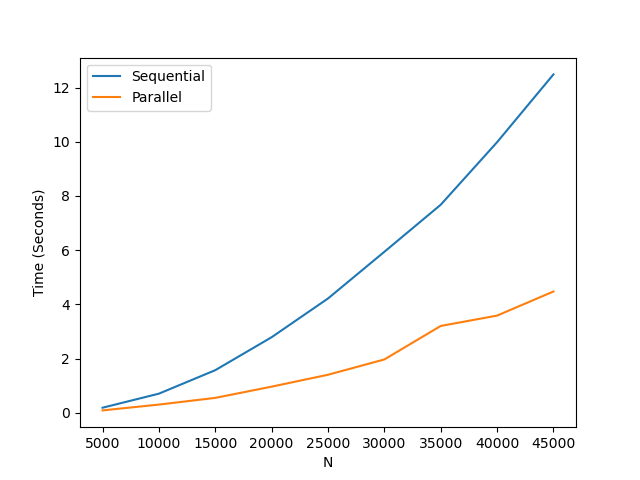
\includegraphics[width=9cm]{images/benchprim8.png}
    \caption{Sequential Prim's vs. Parallel Prim's with 8 threads}
    \label{fig:prim_8_comparison}
\end{figure}
Running the concurrent solution on a 12-core CPU with 8-threads can see that as input sizes grow, the parallel implementation can produce run-times more than 3 times faster than the sequential algorithm.
\begin{figure}[h]
    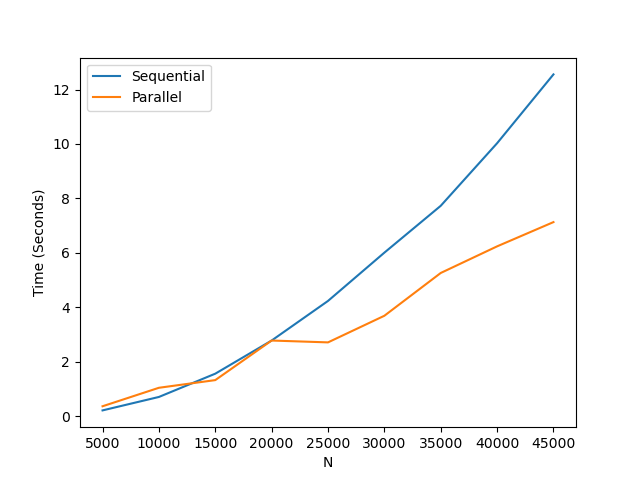
\includegraphics[width=9cm]{images/benchprim12.png}
    \caption{Sequential Prim's vs. Parallel Prim's with 12 threads}
    \label{fig:prim_12_comparison}
\end{figure}
As the data above indicates, as the number of threads reaches the number of cores the runtime improvements become inconsistent, as each shared-memory operation becomes more computationally expensive. Since testing data was limited by CPU cores, it is possible that even further runtime improvements can be observed on CPUs with 16 or more cores and utilizing more active threads.

\section{Single-Source Shortest Path with Negative Edge Weights}
What this bit of the research hopes to address is the problem of finding shortest path distances in a directed weighted graph from a single source with the additional complication of allowing negative edge weights. We will also address the problem of finding negative sum cycles in such graphs. The two most known algorithms that are applicable to this problem are the Bellman-Ford algorithm and the Floyd-Warshall algorithm. We will explore the parallelization of these algorithms in relation to this problem and their performance.

\subsection{The Bellman-Ford Algorithm}\label{AA}

The Bellman-Ford algorithm is designed to find the shortest path from a single source in a general weighted graph G consisting of a vertex set V and an edge set E. The algorithm is also useful for finding negative cycles that are reachable from the source provided.

It relies on the principle that if all of the edges of of non-negative weight, then a shortest path from the source to some vertex will travel through at most V distinct vertices, and therefore at most V - 1 distinct edges. The algorithm works as follows: initially, a distance array will be set up to store the distance from the source to every other vertex. This distance array will be initially filled with an arbitrarily large value, signifying that we have not found a path from the source to this vertex. The source's distance will then be set to 0. Then, a certain number of iterations will be performed. In a single iteration, every edge will be considered in an arbitrary order, and an update for each edge will take place. For some edge from vertex u to vertex v with weight w, if there exists a path from the source to u that has been found (the distance to u is currently less than our arbitrarily large value), and if the distance from u plus the weight w is less than the currently stored distance to v (or if no path to v from the source has been discovered), then the distance to v will be updated. Then, since for any vertex some shortest path will consist of at most V - 1 edges, then the most number of iterations needed in the worst case is exactly V - 1. Some basic C++ code for this step of the algorithm is provided below:

\lstinputlisting[
    language=C++,
    caption=,
    label=
]{./src/negative_edge_weights/bellman_ford.cpp}

The next step of the algorithm deals with handling negative sum cycles in the graph. If there is a negative sum cycle in the graph that is reachable from the source, then every node that exists in the cycle will have an indefinitely small shortest path to it. This is because if the cycle has negative sum to traverse the whole cycle, then for any shortest path of sum X, the cycle could be traversed exactly one more time to achieve a shortest path of sum less than X. This is true for any X, therefore the shortest path sum is undefined for these nodes. This proof expands to all nodes that are even reachable by some node on the negative cycle, even if the path from the cycle to the desired node is positive as an infinitely small sum is achievable in the cycle.

To detect this, only a single more iteration of the edge updating process needs to be done. If it is found that a vertex has a shorter distance now after this iteration, then it must be a part of a negative cycle reachable from the source. These nodes will be marked during this process. Then, a multi-source breadth first search algorithm will be performed with the set of sources as the initially marked nodes. The search will mark all nodes that are reachable from the initially marked nodes. At the end of this process, a node being marked signifies that its minimum sum path from the source to itself is infinitely small. An arbitrarily small value can be set in the distance array to show this. Note that some nodes can have negative shortest path distances without being infinitely negative. Some simple code to find these nodes is shown below:

\lstinputlisting[
    language=C++,
    caption=,
    label=
]{./src/negative_edge_weights/negative_cycle_detection.cpp}

The overall run time for this complete algorithm is O(V * E). It can be seen that the major bottleneck of the algorithm is looping through each edge V - 1 times. The additional Breadth-First-Search at the end to find the special marked nodes is a run time of O(V + E), so the focus of parallelization on the algorithm will be directed towards this O(V * E) double for loop. It is imperative that all edges perform an update on our distance array for one iteration before any edges of the next iteration perform an update. A naive approach to a parallelization of these updates can therefore be as follows: a single parent thread will loop for each iteration of edge updates. Then, the edge updates will be divided evenly among the worker threads. each thread will loop over its selected section of edges, and prepare to make an update for each edge. For some edge from vertex u to vertex v with weight w, the thread will need to make sure while reading the distance table at u and writing to the distance table at vertex v that no other thread modifies these values. A simple fix to this problem is to create a lock for each vertex. When a thread goes to read/modify these values, it locks the two locks for these vertices, then performs the check and update, and then unlocks these locks. Some example C++ code is shown below:

\lstinputlisting[
    language=C++,
    caption=,
    label=
]{./src/negative_edge_weights/bellman_ford_parallel_deadlock_floop.cpp}

\lstinputlisting[
    language=C++,
    caption=,
    label=
]{./src/negative_edge_weights/bellman_ford_parallel_deadlock_thread_stuff.cpp}

The first thing that can be noted about this implementation is that the locks will block the threads quite frequently. A good portion of the time, a thread will be waiting for a lock to unlock before it can make a check/update. This causes a significant loss of efficiency. Not only this, but this implementation also opens up the possibility of deadlock. Since each thread will attempt to lock two different threads sequentially, a situation could arise in which one thread takes a resource needed by another at the same time the other thread takes the resource now needed by the original thread. Then both threads would hang, waiting on each other to give up access to the needed resources.

Both of these issues can be avoided by making the distance array an array of atomic integers. This allows threads to atomically read the distances to the vertices to check if an update is needed, and also atomically write new distances for needed updates. The updated code is shown below:

\lstinputlisting[
    language=C++,
    caption=,
    label=
]{./src/negative_edge_weights/bellman_ford_parallel_better.cpp}

This removes the need for locks offering better performance. One final issue that can be noted is the recreation and destruction of all threads at the end of each iteration. These operations are expensive. Rather than recreating all threads and joining them at the end of every iteration, they can be created all at once and communicate with each other. What needs to be maintained is that all edge relaxations from one iteration be conducted before any of the next. The threads can therefore signal if they are working or waiting for all other threads to wrap up their computations for this current iteration. This can be done by counting the number of currently working threads via an atomic integer. When a thread is entering its workload, it adds one to the counter. Then, when it has finished, it decrements this counter and waits for all other threads to be finished. It will know everyone is done when the counter reaches 0. A simple implementation is shown below:

\lstinputlisting[
    language=C++,
    caption=,
    label=
]{./src/negative_edge_weights/thread_creation_final.cpp}

\lstinputlisting[
    language=C++,
    caption=,
    label=
]{./src/negative_edge_weights/bellman_ford_parallel_final.cpp}

After the running of benchmarks, The only comparable parallelization implementation is the final implementation. The first two implementations struggled to show any efficiency improvements on specific graphs, and ended up being dramatically slower on large graphs due to the locking and thread creation issues mentioned earlier. The final and best implementation with 10 concurrent threads performed well. On average in very large random graphs, the algorithm is about two to three times faster in practice than the standard single-threaded algorithm.

\section{The Disjoint Set Union Problem}

\subsection{Problem Definition}
The Disjoint Set Union, alternatively called the Union Find Problem, is to maintain several disjoint sets with the ability to merge these disjoint sets together and determine if different items are in the same set. This can be achieved by maintaining a unique representative for each disjoint set. When we union two sets, we make the representative of one set the representative of the other set, thus uniting the sets into one.

Such a data structure that can do this should support the following operations: \\ \\
$find(x)$: Find and return the representative of the set that contains $x$. \\ \\
$unite(x, y)$: Get the representative of the set containing $x$ and the representative of the set containing $y$. If the representatives are the same, they are in the same set, otherwise, combine the sets by setting the representative of one of the two representatives to the other. \\ \\
All sets begin only containing it's index, with it's representative being the index. We will also include the following operations: \\ \\
$sameSet(x, y)$: Determine if $x$ and $y$ are in the same set by getting their respective representatives and comparing if they are the same or not.

\subsection{Sequential Implementations}

We will examine naïve implementations of $find(x)$ and $unite(x, y)$, and go over the different optimizations that can be applied to them to improve overall time complexity. As we go along the path of representatives, we will call the next representative the parent, and the representative of the set the root.

\lstinputlisting[
    language=C++,
    caption={Naïve implementation of $find(x)$.},
    label=lst:naivefind
]{./src/disjoint_set_union/dsu_find.cpp}

\lstinputlisting[
    language=C++,
    caption={Naïve implementation of $unite(x, y)$.},
    label=lst:naiveunite
]{./src/disjoint_set_union/dsu_unite.cpp}

These implementations have problems because we have no rules on how we designate who becomes the root of who. We can see here that in the worst case, we can create a long chain of parents, which would make the worst case of $find(x)$ be $O(n)$, with no improvements to happen over time. There are several optimizations that we can do to improve the time complexity. We will first look at linking by size, linking by rank, and linking by random index.

When we link by size, the idea is to maintain the size of each disjoint set, and use the sizes to determine what the new root will be in $unite(x, y)$. When we go to try and unite the two sets, we will make the root of the set that has a larger size be the root of the new combined set. Ties are broken arbitrarily.

\lstinputlisting[
    language=C++,
    caption={Implementation of $unite(x, y)$ with linking by size.},
    label=lst:unitelinkbysize
]{./src/disjoint_set_union/dsu_unite_link_by_size.cpp}

When we link by rank, the idea is to maintain the length of the longest path from the root to any other value in the set. When we $unite(x, y)$, we make the root with the higher rank the root of the new combined set. If there is a tie, we arbitrarily choose the root of the new set, and increase the rank by 1.

\lstinputlisting[
    language=C++,
    caption={Implementation of $unite(x, y)$ with linking by rank.},
    label=lst:unitelinkbyrank
]{./src/disjoint_set_union/dsu_unite_link_by_rank.cpp}

When we link by random index, the idea is to create a random ordering of the values, and use the position in the ordering to determine who becomes the root. The root with the later position in the ordering becomes the root of the combined set. Since each position is unique, there will never be ties.

\lstinputlisting[
    language=C++,
    caption={Implementation of $unite(x, y)$ with linking by random index.},
    label=lst:unitelinkbyrandomindex
]{./src/disjoint_set_union/dsu_unite_link_by_random_index.cpp}

Another point of improvement that can be made is that if the parent of $x$ is $y$ and the parent of $y$ is $z$, since we only care about the root of the whole set, we can get rid of this chain by simply making it so that parent of $x$ is $z$. There are several optimizations for achieving this, being compression, halving, and splitting.

When we do compression, we simply make all the parents on the path are set to the root.

\lstinputlisting[
    language=C++,
    caption={Implementation of $find(x, y)$ with compression.},
    label=lst:findcompression
]{./src/disjoint_set_union/dsu_find_compression.cpp}

When we do halving, we replace the parent of every node on the path with it's grandparent.

\lstinputlisting[
    language=C++,
    caption={Implementation of $find(x, y)$ with halving.},
    label=lst:findhalving
]{./src/disjoint_set_union/dsu_find_halving.cpp}

When we do splitting, we replace the parent of every other node on the path with it's grandparent.

\lstinputlisting[
    language=C++,
    caption={Implementation of $find(x, y)$ with splitting.},
    label=lst:findsplitting
]{./src/disjoint_set_union/dsu_find_splitting.cpp}

\begin{thebibliography}{00}
\bibitem{b1}Seo, Jarim. “Parallel Implementation of a Minimum Spanning Tree Algorithm.” SEO-THESIS-2020, Texas State University, Dec. 2020, https://digital.library.txstate.edu/bitstream/handle/10877/12921/SEO-THESIS-2020.pdf?sequence=1\&amp;isAllowed=y. 
\bibitem{b2}“Prim's Minimum Spanning Tree (MST): Greedy Algo-5.” GeeksforGeeks, 18 Jan. 2022, https://www.geeksforgeeks.org/prims-minimum-spanning-tree-mst-greedy-algo-5/. 

\bibitem{b3}Graves, Jeffrey A. Parallelizing Single Source Shortest Path with OpenSHMEM. United States: N. p., 2017. Web.

\end{thebibliography}

\end{document}